\section{System architecture}\label{5_3_systemArchitecture}
%- System architecture of system --> Unity3D, Kinect SDK, Kinectstudio, VGB --> kinect sdk free to use since version X
In the following several components of the general system architecture will be described that are necessary for the functionality of the interactive learning system with real-time feedback and for the study afterwards. An overview can be seen in figure~\ref{fig:5_3_systemArchitecture}.
\begin{figure}[htb]
	\centering
	\begin{minipage}[t]{1\linewidth}
		\centering
		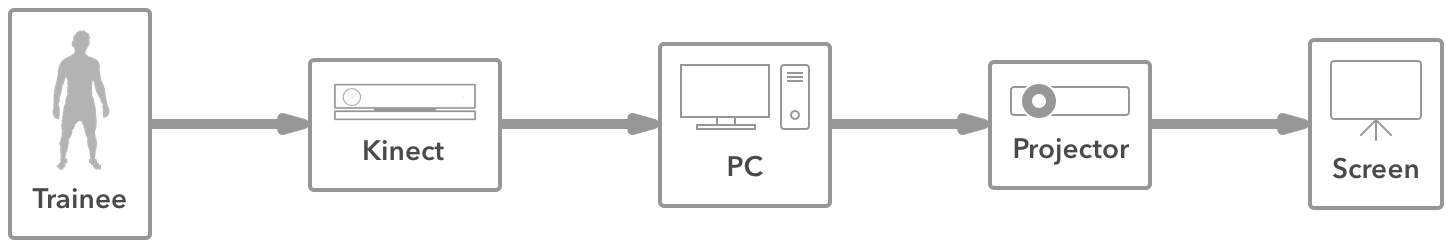
\includegraphics[width=1\linewidth]{Pictures/5_3_systemArchitecture}
		\caption{System overview}
		\label{fig:5_3_systemArchitecture}
	\end{minipage}
\end{figure}

\subsection{Hardware and software components}
% Kinect, Beamer, Screen, Slackline --> Alpidex High Performance

As slackline the mobile \textit{alpidex POWER-WAVE 2.0} is used. It is placed in front of the \textit{Microsoft Kinect v2}, which is used as tracking device. The Kinect itself is attached on a \todo{modell} tripod with a height of about \todo{height, hüfthöhe?}. A \textit{Steambox PC} \todo{footnote specs} served as development device that fulfilled the recommended specs of the Kinect: \textit{Windows 8, 4 GB Memory, Physical dual-core processor with 3.1 GHz or faster, USB 3.0 Gen-2 controller, Graphics card supporting DirectX 11}. A projector \todo{modell} with a resolution of 1920x1080 was attached on a traverse system to give the user a more immersive feeling. The image is visualised on a projection screen with a size of \todo{2x3m}.

% KinectStudio, VGB, Unity3D, Kinect SDK for unity, Kinect MS-SDK
For software realization the cross-platform game engine \textit{Unity3D} by \textit{Unity Technologies} is used. It is widely known for developing games but manufacturer of several interaction devices (e.g. \textit{HTC Vive}, \textit{Oculus Rift}, \textit{Leap Motion}) provide \todo{compatibility packages} to make use of them in Unity. Applications can be deployed for several platforms on desktop, mobile, web, console, TV, VR, and AR (e.g. Windows, macOS, Android, iOS, Oculus Rift, Windows Mixed Reality and so on).

To access the data stream of the Kinect the \textit{Microsoft Kinect SDK v2.0}~\footnote{\label{fn:kinectTools}\url{https://developer.microsoft.com/de-de/windows/kinect/tools}} has to be installed on the PC. Microsoft offers also a \textit{Kinect for Windows Unity package}\cref{fn:kinectTools}, which provides all required scripts in Unity for creating a Kinect based unity application. Since \textit{Unity 5} it can be used with the free personal edition of Unity, whereas before it could be only used with the pro version. Also the \textit{Kinect v2 Examples with MS-SDK} \footnote{\url{https://www.assetstore.unity3d.com/en/\#!/content/18708}} by Rumen Filkov was used to make data access and interaction implementation more simple as well as getting an idea on how to handle incoming data from the Kinect.

\todo{hier evtl UI design chapter rein}

\subsection{Implementation}
The software development process consists of the interplay of two system components (Figure~\ref{fig:5_3_unityKinectArchitecture}). First Unity itself, which is used to create the virtual environment, interface, and manage actions by the user. Second the Kinect SDK plugin for accessing input data of the user recognized by the Kinect device like e.g. joint position, gesture detection, and user actions. In the following the data structure and management, interaction integration, and feedback implementation of the system are further described.
\begin{figure}[htb]
	\centering
	\begin{minipage}[t]{1\linewidth}
		\centering
		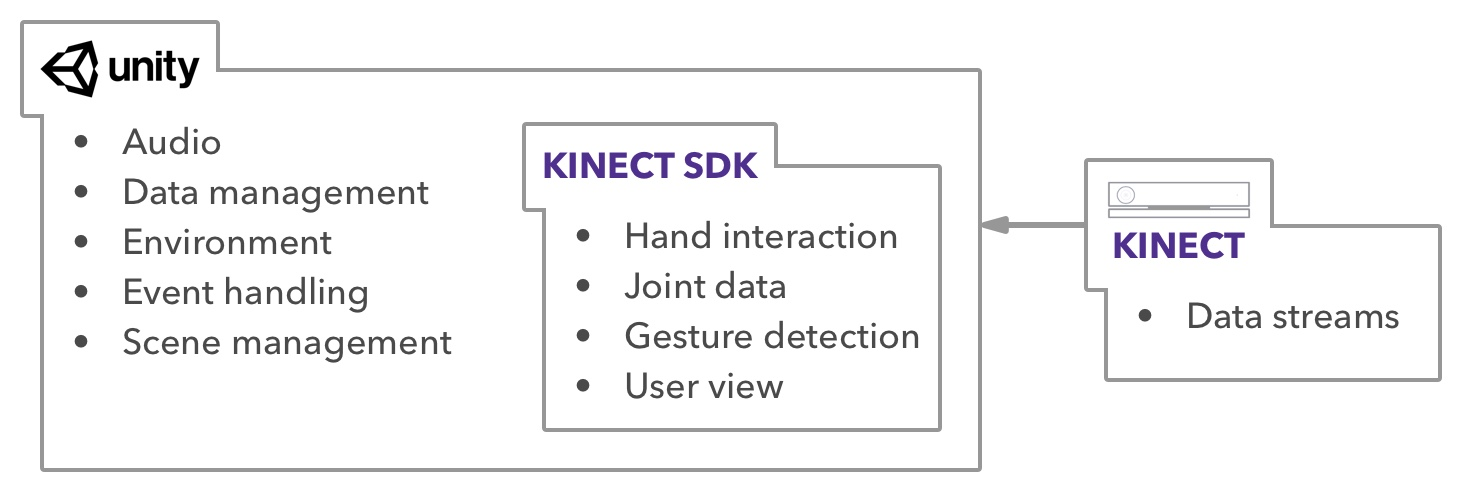
\includegraphics[width=1\linewidth]{Pictures/5_3_unityKinectArchitecture}
		\caption{Unity and Kinect architecture}
		\label{fig:5_3_unityKinectArchitecture}
	\end{minipage}
\end{figure}

%This application a 3D project has been generated, since the Kinect uses 3D space to track the user, she should be able to interact within that, and a 3-Dimensional environment design is considered. Further some examples of the interaction implementation is described.
\subsubsection{Data management}
All relevant user and exercise data will be stored in JSON files, which is more human-readable and makes accessing and updating data simple in Unity via the JSON serialization feature~\footnote{\url{https://docs.unity3d.com/Manual/JSONSerialization.html}}. Each user should have the same basement regarding the exercises. Therefore a default exercise JSON file serves as reference for all registered users in the system. An internal editor for exercises and users was created for proper data management and to adjust the data files more easily for testing purposes. The overall data structure can be seen in figure \todo{img ref data structure}.

%For each object containing key-value pairs a class is generated, i.e. for Users, Tier, Exercise, Sides, and Repetitions. In listing \todo{ref c\# code example} an example for the \textit{Tier} object can be seen. A class must be marked as serializable to work with the JSON serializer. It contains variables, which match the JSON structure on listing \todo{ref json code}. 
%\todo{c\# code example and json file}

%With this an instance of the class can be created and the value accessed for adjustments (listing \todo{ref img class instance}). This can then be serialized into a JSON object. Line \todo{ln number} shows how existing JSON data can be converted back into an object instance. This is needed to fetch user data that already exists.

%\todo{img class instance}


%\todo{img editor window}

%The files are stored within the \textit{StreamingAssets} folder of Unity. Data stored in this folder can easily be accessed via path name of the target machines file system. 

\todo{image of data structure}

\subsubsection{Engagement gesture}
The engagement gesture is the very first user interaction with the system. %It is done by raising any hand over the head. This is to convey her that the system recognises specific movement actions. 
She has to raise her hand over the head whereupon the system conveys that it recognises specific user actions. 

A code example on how to this gesture is implemented can be seen in listing~\ref{lst:codeEngagement}.
%The \textit{KinectManager} exists as an empty \textit{GameObject} in the scene and has to be referenced in the script. The \textit{KienctInterop} class delivers several utility and interop function and calls the sensor interfaces. Here it is used to assign the proper joint type for tracking them. 
First the developer has to assure that the Kinect is initialized, a user has been detected, and the relating joints are recognized.  A condition checks if the current vertical position of the right hand is above the head joint (\textit{Listin~\ref{lst:codeEngagement} line~\ref{lst:codeEngagement15}}). If this is the case, the next scene can be loaded. 
%This is actually part of the script for the first scene in the application, in which the user has to engage with the Kinect by doing the described movement.

\begin{lstlisting}[caption=C$^\sharp$ example code for tracking a raising hand, label=lst:codeEngagement]
if (_kinectManager.IsInitialized() && _kinectManager.IsUserDetected())
{
	long uId = _kinectManager.GetPrimaryUserID();

	if ((_kinectManager.IsJointTracked(uId, (int) _jointHandRight) && 
			 _kinectManager.IsJointTracked(uId, (int) _jointHead))
	{
		Vector3 jointHandRightPosition = 
			_kinectManager.GetJointKinectPosition(uId, (int) _jointHandRight);
		Vector3 jointHeadPosition = 
			_kinectManager.GetJointKinectPosition(uId, (int) _jointHead);			

		if (jointHandRightPosition.y > jointHeadPosition.y)(*@ \label{lst:codeEngagement15} @*)
			SceneManager.LoadScene("Tutorial");
	}
}
\end{lstlisting}

\begin{comment}
\begin{lstlisting}[caption=C$^\sharp$ example code for tracking a raising hand, label=lst:codeEngagement]
public  KinectManager KinectManager;
private KinectManager _kinectManager;
private KinectInterop.JointType _jointHandRight, _jointHead;

void Start ()
{
	_jointHandRight = KinectInterop.JointType.HandRight;
	_jointHead = KinectInterop.JointType.Head;
}
void Update ()
{
	if (KinectManager == null) return;
	_kinectManager = KinectManager.GetComponent<KinectManager>();

	if (_kinectManager && 
		  _kinectManager.IsInitialized() && 
		  _kinectManager.IsUserDetected())
	{
		long uId = _kinectManager.GetPrimaryUserID();

		if ((_kinectManager.IsJointTracked(uId, (int) _jointHandRight) && 
			   _kinectManager.IsJointTracked(uId, (int) _jointHead))
		{
			Vector3 jointPosHandRight = 
			 _kinectManager.GetJointKinectPosition(uId, (int) _jointHandRight);
			Vector3 jointPosHead = 
			 _kinectManager.GetJointKinectPosition(uId, (int) _jointHead);			

			if (jointPosHandRight.y > jointPosHead.y)(*@ \label{lst:codeEngagement15} @*)
				SceneManager.LoadScene("Tutorial");
		}
	}
}
\end{lstlisting}
\end{comment}

\subsubsection{Hand cursor interaction}
To provide the possibility of an autonomous interaction the user has to navigate on her own with the system. Her hands serve as input for interacting with interface elements. The current position on the screen is visualised by a virtual cursor. Therefore she is in constant interaction with the system and becomes more familiar to it.

Four different approaches were tested as interaction gesture. First hovering with the hand over elements (Figure~\ref{fig:5_3_hover}). It is a good approach if small elements should be selectable. However relatively big and many interaction elements exists in the system, which resulted in accidental and unwanted misclicks.
The second one is interacting by closing the hand to a fist or grab gesture and releasing it(Figure~\ref{fig:5_3_fist}). This resulted also in unwanted misclicks because of the anatomical behaviour and tracking distance. The hand of the testing users closes automatically a little bit during system interaction, which is sufficient to trigger a click (Figure \todo{comparison default \& target }).
A better interaction gesture is the \textit{V-sign}. The user makes simply a pointing gesture with the index as well as the middle finger. The click event triggers when the user releases her hand into the default state (Figure~\ref{fig:5_3_point}). The last interaction gesture is pushing the hand towards the Kinect. It is related to the real world like pushing a button down and therefore the most intuitive and natural gesture behaviour (Figure~\ref{fig:5_3_push}). %Since in this gesture the hand has to move from point a to point b in the z-axis the progress is visualized by a filling circle like seen in figure~\ref{fig:handcursorProgress}.

Therefore as main interaction serves the hand push gesture. The V-sign servers as fallback interaction if something wents wrong with the push gesture.

\begin{figure}[htb]
	\centering
	\begin{minipage}[t]{0.15\linewidth}
		\centering
		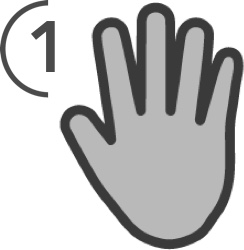
\includegraphics[width=1\linewidth]{Pictures/5_3_hover}
		\subcaption{Hover and wait}
		\label{fig:5_3_hover}
	\end{minipage}
	\hfill
	\begin{minipage}[t]{0.1\linewidth}
		\centering
		
\includegraphics[width=1\linewidth]{Pictures/5_3_fist}
		\subcaption{Grab}
		\label{fig:5_3_fist}
	\end{minipage}
	\hfill
	\begin{minipage}[t]{0.12\linewidth}
		\centering
		
\includegraphics[width=1\linewidth]{Pictures/5_3_point}
		\subcaption{Lasso}
		\label{fig:5_3_point}
	\end{minipage}
	\hfill
	\begin{minipage}[t]{0.22\linewidth}
		\centering
		
\includegraphics[width=1\linewidth]{Pictures/5_3_push2}
		\subcaption{Pushing towards Kinect}
		\label{fig:5_3_push}
	\end{minipage}
	\caption{Several tried hand interaction techniques of the Kinect}
	\label{fig:5_3_handInteraction}
\end{figure}

\begin{comment}
\begin{figure}[htb]
	\centering
	\begin{minipage}[t]{1\linewidth}
		\centering
		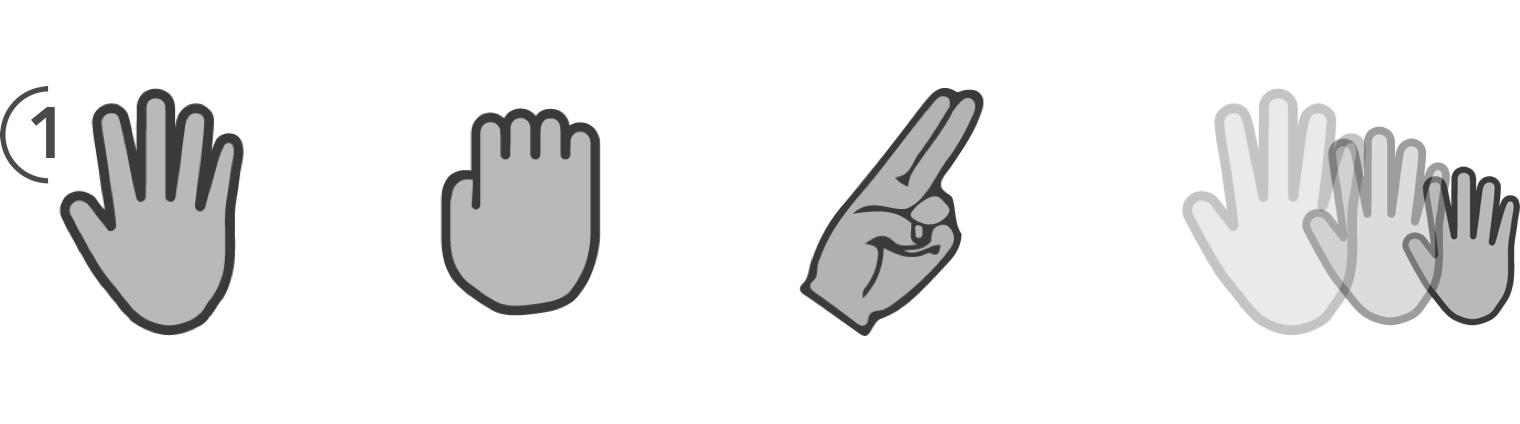
\includegraphics[width=1\linewidth]{Pictures/5_3_handInteraction}
		\caption{Several hand interaction techniques of the Kinect}
		\label{fig:5_3_handInteraction}
	\end{minipage}
\end{figure}

\begin{figure}[htb]
	\centering
	\begin{minipage}[t]{1\linewidth}
		\centering
		
\includegraphics[width=0.6\linewidth]{Pictures/handcursorProgress}
		\caption{Progress of handcursor (Left: Default, Middle: In progress, Right: Finished)}
		\label{fig:handcursorProgress}
	\end{minipage}
\end{figure}
\end{comment}

\subsubsection{Starting position}\label{5_2_1_startingPosition}
After engaging with the system the user is introduced on how to stay in a proper starting position. She has to stand with both feet parallel and in front to the Kinect like in figure \todo{ref illustration}. This is required by some actions like just before starting the exercise execution. It ensures the readiness of the user and is needed to get the initial foot joint positions (cf. \todo{section Feedback integration}). This is mainly to verify that the user stays, in the slackline exercises, on the line and not on the ground, since the Kinect cannot cover this condition.
%This initial joint position can differ if the user stands closer or more far away from the sensor because of the Kinects angel regarding its height. Hence the z-axis joint position of the left and right feet will be compared to have the same value with a little tolerance. 

\todo{illustration feets parallel}

\subsubsection{User selection}
The system can have multiple user profiles. Hereby more than one user can train with the system separately. When the trainee selects her profile the system checks if the JSON file has any data. If no data is available, which means it is a new user, the default exercise JSON file will be copied into the profile. Then all exercise data are loaded into the system for data adjustment and management.
%The trainee selects her profile by herself. With this the data will be loaded into the system. In the user selection the trainee should select the right profile by herself to cover the condition of multiple user that can train with the system. 
%The users name and id are saved in as \textit{PlayerPrefs}. This is a class in Unity that provides the possibility to be globally accessible in the application. The respective code for setting and getting the values can be seen in listing \todo{ref listing playerpfrefs}. This is needed to find the correct path for the JSON files to save the data.

\subsubsection{Tier \& exercise menu}
The tier and exercise menus are designed as levels. Like a regular level system all levels are locked but the first one to provide a starting position. They can be unlocked by executing each exercise of the previous one. The structure already seen in section \textit{\ref{4_4_exercises}} is adapted to store the corresponding information for the tier, exercise, side, and repetition.

\subsubsection{Exercise execution, providing feedback}
The exercise execution consists of the biggest functionality implementation. Feedback indicators provide the user with necessary information about the current exercise in real time. This should help to enhance the performance in her execution and for successfully accomplishing the exercise. In the slackline system the following feedback indicators are integrated:

\begin{itemize}
\item Correct performance of an exercise
\item How good the exercise is currently performed, namely the confidence
\item Elapsed time the user is performing the exercise
\item When the repetition was successful (i.e. minimum time has been reached)
\item When a repetition attempt was not successful
\item Amount of repetitions in general, finished, and left
\item Checklist about key elements of an exercise (hands up, foot stretched, etc.)
\end{itemize}

After each successful exercise execution the user is lead to a summary screen. Here she gets an overview about her performance. It shows parameters about the execution time, attempts, and the confidence for each repetition as well as an average value for the accomplished side. A similar summary screen exists also for the entire level with the same parameters but only the average value for the entire exercises.

\begin{comment}
\item When an exercise is currently correctly performed
\item How good the exercise is currently performed, namely the confidence
\item The elapsed time the user is performing the exercise
\item When the repetition is successfully accomplished, i.e. the minimum time has been reached
\item When an repetition attempt was not successful
\item How many repetitions in general, finished and left
\item Checklist about key elements in an execution (like hands up, foot stretched, etc.)
\item A summary that shows the user parameters about the performance (execution time, overall attempts, confidence) for each repetition and an average value of these
\item A similar summary can also be found for the entire stage, where the same parameters for each exercise are listed in average
\end{comment}